\section{Prefix-free graphs}
The idea of prefix-free graphs is inspired by a technique used in the tool rsync named Context-Triggered Piecewise Hashing (CTPH) \cite{kornblum2006identifying}.
CTPH uses a rolling hash to partition a string into substrings such that long repeated substrings are partitioned the same way.
These substrings are then hashed with a traditional hash function and stored as a string signature.
The signatures of several files are then compared to determine changes.

In prefix-free graphs, we partition each sequence of a given pangenome into \emph{segment}s.
These segments form nodes of the prefix-free graph, and their adjacencies in the original sequences constitute edges.
The sequences are represented as \emph{path}s in the graph.

The segments have two essential characteristics making them a good choice for nodes of a pangenomic graph.
Similarly to CTPH, long repeated sequences will be partitioned the same way.
Furthermore, no segment is a prefix of another, making a set of segments prefix-free.
The second characteristic is crucial for connecting prefix-free graphs and suffix arrays, as will be presented in the next section.

To create a prefix-free graph from a given pangenome $P$, we define a set of trigger words $T$, where each trigger word is a string of length $k$.
For this set $T$, we build an Aho-Corasick automaton \cite{aho1975efficient}.
Then, for each sequence in pangenome $P$, we append $k$ sentinel characters and iterate over such modified sequence, searching for matches with set $T$ using the automaton.
Each time we encounter a trigger word, we recognize a new segment from the start of the previous trigger word to the end of the current trigger word.
If the segment's sequence was not yet observed during the scan, we add it to the set of segments and assign a unique ID.
Each time we append the corresponding ID to the path representing the original sequence. 

Two special cases happen during the sequence scan, one at the beginning, when no previous trigger word was encountered, and another at the end, when the last $k$ characters are sentinels.
These are addressed by simply starting the first segment at the start of a sequence and ending the last at the sequence end.

Notably, the adjacent segments overlap by exactly $k$ characters.
Furthermore, trigger words occur only at the beginnings or ends of segments because any occurrence of a trigger word in the middle of a segment would break it into two.
This feature and the choice of sentinels outside the sequence's alphabet guarantee that the set of segments is prefix-free.
A sketch of the proof is shown in Figure \ref{fig:proof}.

\begin{figure}
    \centering
    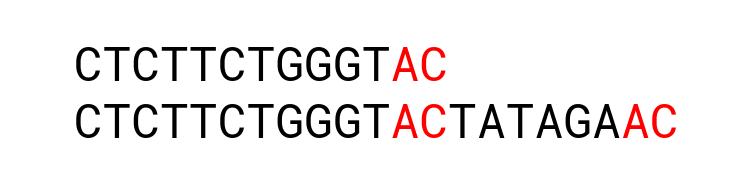
\includegraphics[width=0.6\linewidth]{images/prefixfree_proof.png}
    \caption{
        A sketch of a visual proof that the trigger words induce prefix-free segments.
        Suppose a segment is a prefix of another segment.
        By construction, it ends with a trigger word.
        This trigger word would be in the middle of another segment and would break it into two smaller segments.
    }
    \label{fig:proof}
\end{figure}

After the previous steps, the set of segments and the list of paths already represent a prefix-free graph.
However, to simplify the usage of prefix-free graphs, we recommend normalizing them.
During the normalization, we sort segments lexicographically and change their IDs to correspond to the lexicographical ranks.
This relabeling is then also propagated to paths accordingly. 

To illustrate the entire procedure, consider a set of sequences $P = \{$\texttt{CACGTACT}, \texttt{CACACT}, \texttt{CACGACT}$\}$ and a set of trigger words $T = \{$\texttt{AC}, \texttt{CG}$\}$.
After the partitioning, we obtain a set of segments with IDs $\{$\texttt{0:CAC}, \texttt{1:ACG}, \texttt{2:CGTAC}, \texttt{3:ACT..}, \texttt{4:ACAC}, \texttt{5:CGAC}$\}$ and a list of paths \texttt{[[0,1,2,3], [0,4,3], [0,1,5,3]]}.
After the normalization, we get a prefix-free graph which can be directly represented in GFA format as shown in Figure \ref{fig:gfa}.

\begin{figure}
    \centering
    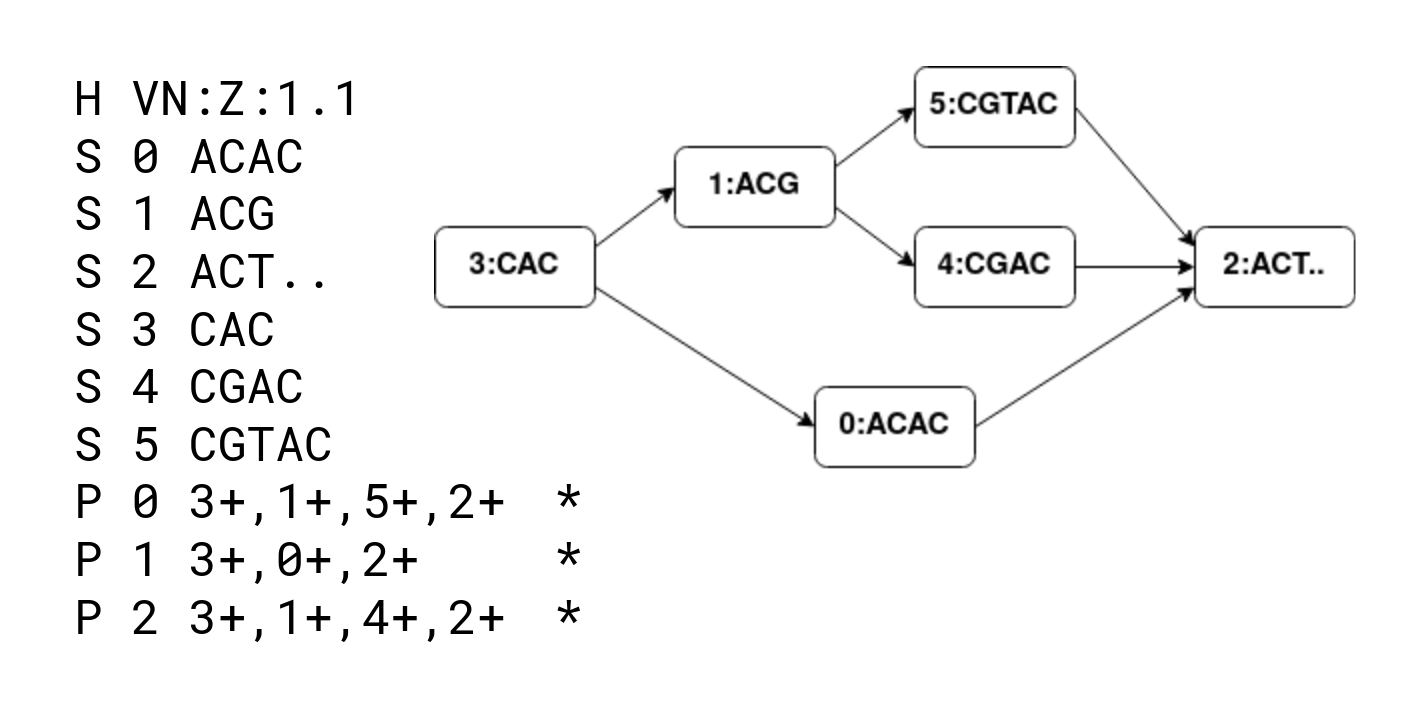
\includegraphics[width=\linewidth]{images/pfg_gfa.png}
    \caption{
        Prefix-free graph of the running example after normalization and its representation in GFA format.
        Link lines omitted for brevity.
    }
    \label{fig:gfa}
\end{figure}

From this representation, original sequences of a pangenome can be reconstructed by expanding the segment IDs in a particular path, ignoring the last $k$ characters of each segment.

